\documentclass[11pt,letterpaper]{article}
\PassOptionsToPackage{hyphens}{url}
\usepackage[margin=.83in,top=.8in,bottom=.8in,headheight=15pt]{geometry}
\usepackage[T1]{fontenc}
\usepackage{lmodern,amsmath,amssymb,mathtools,bm,booktabs,array,graphicx,tikz}
\usetikzlibrary{arrows.meta,positioning,calc,decorations.pathreplacing,patterns}
\definecolor{ink}{HTML}{17344D}\definecolor{accent}{HTML}{087E8B}\definecolor{pale}{HTML}{EDF5F5}\definecolor{gold}{HTML}{AD6B19}
\providecommand{\dd}{\,\mathrm{d}}\providecommand{\R}{\mathbb{R}}
\providecommand{\E}{\mathbb{E}}\providecommand{\Var}{\operatorname{Var}}
\providecommand{\Cov}{\operatorname{Cov}}\providecommand{\diag}{\operatorname{diag}}
\providecommand{\norm}[1]{\left\lVert#1\right\rVert}
\providecommand{\abs}[1]{\left|#1\right|}
\usepackage{microtype,hyperref,fancyhdr,enumitem,amsthm,sectsty,needspace}
\allsectionsfont{\raggedright}
\hypersetup{colorlinks=true,linkcolor=ink,urlcolor=accent,pdfauthor={Zan Ahmad},pdftitle={Regression, classification, and multivariate data / Lecture notes}}
\setlength{\parindent}{0pt}\setlength{\parskip}{6pt}\linespread{1.07}
\setlist{itemsep=3pt,topsep=4pt,leftmargin=*}
\emergencystretch=2em\clubpenalty=10000\widowpenalty=10000
\pagestyle{fancy}\fancyhf{}\fancyhead[L]{\small Scientific Computing in Python / 2027}\fancyhead[R]{\small Lecture 4}
\fancyfoot[L]{\footnotesize Zan Ahmad}\fancyfoot[R]{\footnotesize\thepage}\renewcommand{\headrulewidth}{.3pt}
\newtheorem{proposition}{Proposition}\newtheorem{theorem}{Theorem}\newtheorem{lemma}{Lemma}
\theoremstyle{definition}\newtheorem{definition}{Definition}\newtheorem{example}{Example}
\numberwithin{equation}{section}
\begin{document}
{\small\scshape Scientific Computing in Python / 2027\hfill Lecture 4}\par\medskip
{\raggedright\hyphenpenalty=10000\exhyphenpenalty=10000\LARGE\bfseries\color{ink} Regression, classification, and multivariate data\par}\medskip
{\small Lecture notes}\par\bigskip
Synthetic experiments record temperature, duration, and measured yield. Regression estimates yield as a number. Classification estimates a score for reaching a stated yield threshold. Principal components and clustering describe the predictor geometry. We keep the statistical targets and the fitted transformations distinct throughout.

\section{The design matrix}
\hypertarget{note-the-design-matrix}{}\label{note:the-design-matrix}
{\small \href{slides.html\#frame=the-design-matrix\&step=1}{Slides for this section}}\par
Let $T_i$ and $d_i$ be the temperature and duration of experiment $i$, and $y_i$ its measured yield. An affine model uses an intercept and one coefficient for each predictor. The columns of the design matrix have different units; the corresponding coefficients supply the units needed to produce yield.

\[
A=\begin{pmatrix}1&T_1&d_1\\\vdots&\vdots&\vdots\\1&T_n&d_n\end{pmatrix},\qquad
\widehat y=A\beta.
\]

\[
\widehat y_i=\beta_0+\beta_TT_i+\beta_dd_i.
\]

\subsection*{Least-squares equations}
\[
\widehat\beta=\arg\min_\beta\|A\beta-y\|_2^2,
\qquad A^{\mathsf T}(A\widehat\beta-y)=0.
\]

Use a QR/SVD-based solve. An explicit inverse is unnecessary.
\section{A success event}
\hypertarget{note-a-success-event}{}\label{note:a-success-event}
{\small \href{slides.html\#frame=a-success-event\&step=1}{Slides for this section}}\par
Define the actual label from measured yield: $z_i=1$ when $y_i\geq8$ mg. This threshold defines the event to predict. The model's score threshold is a separate choice applied to a fitted probability-like score. Observed yield must not be placed among predictors when the task is to predict success before yield is measured.

\[
z_i=\mathbf1_{\{y_i\geq8\ \mathrm{mg}\}},\qquad
p_i=\sigma(w_0+w_TT_i+w_dd_i).
\]

\[
\widehat z_i=\mathbf1_{\{p_i\geq0.5\}}.
\]

\subsection*{Two distinct thresholds}
The $8$ mg threshold defines the actual scientific outcome.

The $0.5$ score threshold defines the decision rule. Moving the second threshold changes false-positive and false-negative counts without changing the measured labels.
\section{Training-only standardization}
\hypertarget{note-training-only-standardization}{}\label{note:training-only-standardization}
{\small \href{slides.html\#frame=training-only-standardization\&step=1}{Slides for this section}}\par
A predictor with larger numerical units can dominate Euclidean distances and affect gradient-descent scaling. Standardize using training means and standard deviations. The transformation is then frozen for held-out observations. A constant predictor must receive an explicit treatment because its standard deviation is zero.

\[
x'_{ij}=\frac{x_{ij}-\mu_{j,\rm train}}{s_{j,\rm train}}.
\]

The same $\mu_j,s_j$ are used for all later predictions.

\subsection*{Prediction on a new experiment}
\begin{minipage}{\linewidth}
\begin{verbatim}
X_test_scaled = (X_test - train_mean) / train_scale
prediction = model(X_test_scaled)
\end{verbatim}
\end{minipage}

Re-estimating the scale from test rows would change the fitted procedure.
\begin{center}\begin{minipage}{.98\linewidth}\centering
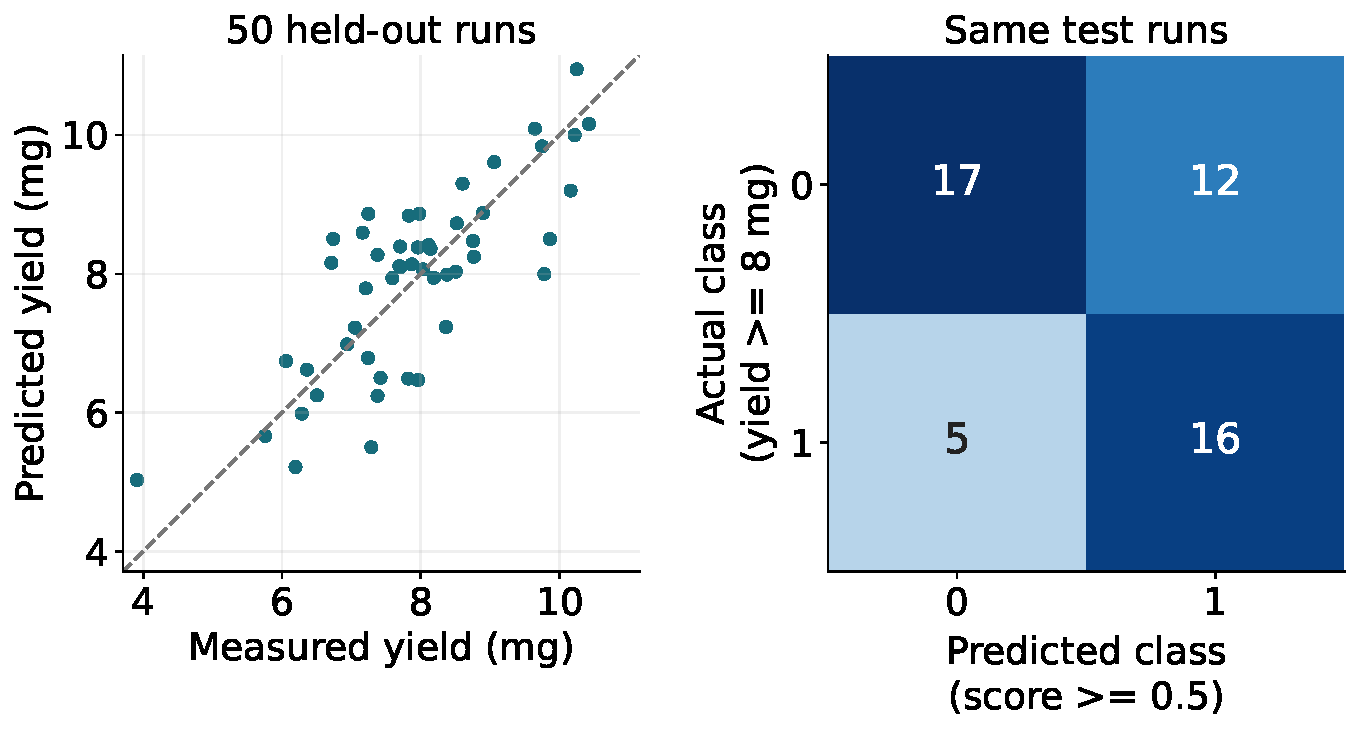
\includegraphics[width=.96\linewidth,height=.57\textheight,keepaspectratio]{heldout-predictions.pdf}\par\smallskip
{\small Both panels use the same 50 held-out synthetic runs. The regression diagonal marks exact agreement. Classification uses measured yield $\geq$8 mg for the actual label and model score $\geq$0.5 for prediction.}
\end{minipage}\end{center}
\section{Regression and classification errors}
\hypertarget{note-regression-and-classification-errors}{}\label{note:regression-and-classification-errors}
{\small \href{slides.html\#frame=heldout-predictions-figure\&step=1}{Slides for this section}}\par
RMSE measures yield discrepancies in milligrams. Classification metrics count threshold decisions. A prediction can have a small yield error yet cross the success boundary, especially near 8 mg. Conversely a large yield error can leave the class unchanged when both values lie far on the same side.

\[
\mathrm{RMSE}=\sqrt{\frac1N\sum_i(y_i-\widehat y_i)^2}.
\]

\[
\mathrm{precision}=\frac{TP}{TP+FP},\qquad
\mathrm{recall}=\frac{TP}{TP+FN}.
\]

\subsection*{Near-boundary observations}
An actual yield of $8.1$ mg and a prediction of $7.9$ mg differ by only $0.2$ mg, but fall on opposite sides of the success threshold.

Report the numerical target and decision target separately.
\section{Principal components}
\hypertarget{note-principal-components}{}\label{note:principal-components}
{\small \href{slides.html\#frame=principal-components\&step=1}{Slides for this section}}\par
Center the training predictor matrix. A first principal direction maximizes projected predictor variance under a unit-norm constraint. It does not use the response labels. Its usefulness for prediction therefore cannot be concluded from the fraction of predictor variance retained.

\[
\max_{\|v\|_2=1}v^{\mathsf T}X_c^{\mathsf T}X_cv,
\qquad X_c^{\mathsf T}X_cv=\lambda v.
\]

The score of a new row is $s=(x-\mu)v_1$.

\subsection*{Reconstruction error}
\[
\widehat x=\mu+sv_1^{\mathsf T}.
\]

The lost component $(x-\mu)-sv_1^{\mathsf T}$ is orthogonal to $v_1$. It may still contain information about yield.
\begin{center}\begin{minipage}{.98\linewidth}\centering
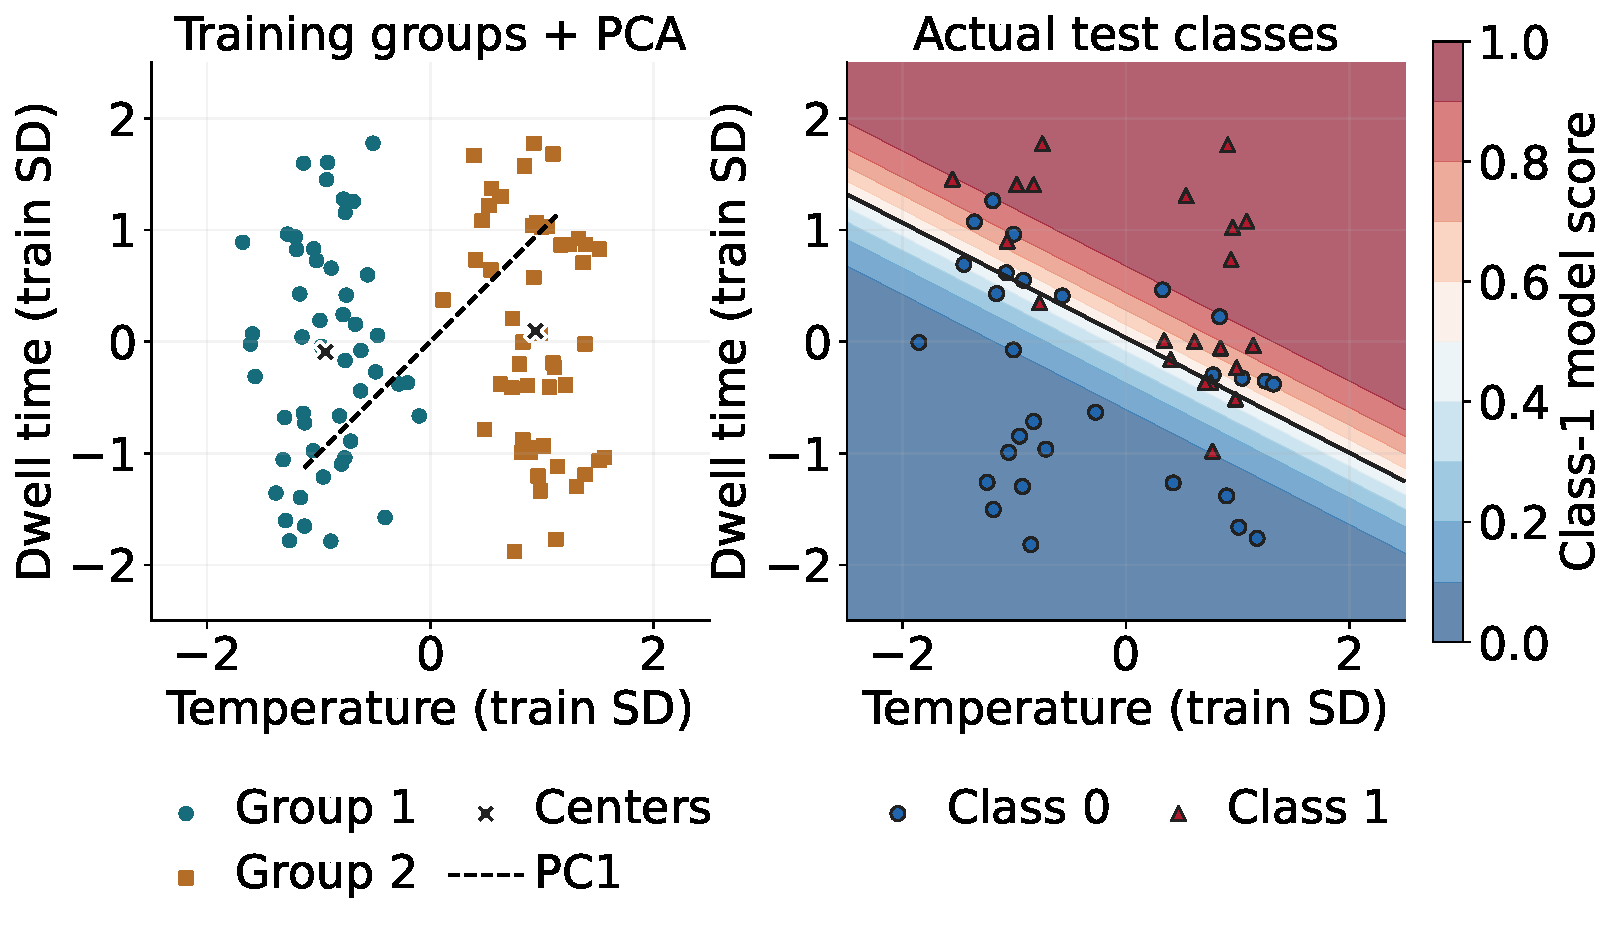
\includegraphics[width=.96\linewidth,height=.57\textheight,keepaspectratio]{presentation-figures/projection-groups-classification.pdf}\par\smallskip
{\small Left colors show training-only two-center memberships and the dashed line marks PC1. Right points show actual test success labels over the fitted logistic score field. The color meanings differ between panels.}
\end{minipage}\end{center}
\section{Distance-based groups}
\hypertarget{note-distance-based-groups}{}\label{note:distance-based-groups}
{\small \href{slides.html\#frame=projection-groups-classification-figure\&step=1}{Slides for this section}}\par
Two-center clustering partitions standardized predictor rows by proximity to fitted centers. The assignments are unsupervised and need not agree with success labels. A graph colored by clusters and a graph colored by actual classes therefore use different meanings of color even if their point locations are identical.

\[
\min_{\mu_1,\mu_2,c_i}\sum_i\|x_i-\mu_{c_i}\|_2^2.
\]

Cluster assignments depend on predictor geometry, not on the success event.

\subsection*{Evaluation after fitting}
Fit scaling, regression, classification, projection and cluster centers using training data.

Evaluate each operation on the held-out experiment using its own stated target. Do not select the best-looking method from repeated test-set inspection.
\bigskip
\section*{Exercises}
\par\noindent\begin{minipage}{\linewidth}
\subsection*{P27-4-1. Define the prediction time}
A different synthetic experiment records pressure before a run and final concentration afterward. Success is final concentration $\geq$6 mg/L. Total: 10 points.

\textbf{a} Identify a regression target, a binary label and one legitimate pre-run feature.

\end{minipage}\par\medskip
\textbf{b} Explain why final concentration cannot also be a legitimate input to a pre-run success predictor.

\textbf{c} If repeated runs share the same specimen, why might a random row split mislead?

\par\noindent\begin{minipage}{\linewidth}
\subsection*{P27-4-2. Compute and compare regression error}
Held-out yields are [4,7,9] mg; model predictions are [5,6,8] mg. A predeclared constant baseline predicts 6 mg for each. Total: 10 points.

\textbf{a} Compute the model residuals as observed minus predicted and its RMSE.

\end{minipage}\par\medskip
\textbf{b} Compute the baseline RMSE and state the bounded comparison.

\textbf{c} What goes wrong if the baseline constant is chosen to minimize error on these same test rows?

\par\noindent\begin{minipage}{\linewidth}
\subsection*{P27-4-3. Read counts before scores}
For a new classifier, actual-by-predicted counts are [[18,2],[6,14]]. Total: 10 points.

\textbf{a} Name TN, FP, FN and TP, then compute accuracy.

\end{minipage}\par\medskip
\textbf{b} Compute precision and recall for class 1 and explain each denominator.

\textbf{c} What is precision if the classifier predicts no positives?

\par\noindent\begin{minipage}{\linewidth}
\subsection*{P27-4-4. Projection and grouping are not labels}
Two standardized input features are projected onto PC1 and grouped by a two-center algorithm. Total: 10 points.

\textbf{a} Does PCA need success labels, and what does its first direction optimize?

\end{minipage}\par\medskip
\textbf{b} A retained component explains 55\% of variance. How much is omitted, and does this quantify prediction accuracy?

\textbf{c} Why can swapping cluster IDs leave the result unchanged? Give one reason the groups may differ from success classes.

\section*{References}
\noindent\begin{minipage}{\linewidth}
Original Python Lecture 5. PDF pages 5--18.

\url{https://zanahmad.com/files/scientific-python/Lecture_5__Intro_to_Python.pdf}
\end{minipage}\par\medskip
\noindent\begin{minipage}{\linewidth}
NumPy least-squares documentation. numpy.linalg.lstsq: minimum residual, rank and singular values.

\url{https://numpy.org/doc/stable/reference/generated/numpy.linalg.lstsq.html}
\end{minipage}\par\medskip
\noindent\begin{minipage}{\linewidth}
Scikit-learn decomposition guide. Section 2.5.1.1: PCA.

\url{https://scikit-learn.org/stable/modules/decomposition.html#pca}
\end{minipage}\par\medskip
\noindent\begin{minipage}{\linewidth}
Scikit-learn clustering guide. Section 2.3.2: K-means and inertia.

\url{https://scikit-learn.org/stable/modules/clustering.html#k-means}
\end{minipage}\par\medskip
\noindent\begin{minipage}{\linewidth}
Scikit-learn model evaluation guide. Binary confusion matrix, precision and recall definitions.

\url{https://scikit-learn.org/stable/modules/model_evaluation.html}
\end{minipage}\par\medskip
\noindent\begin{minipage}{\linewidth}
Scikit-learn common pitfalls guide. Sections 12.1--12.2.1: preprocessing and data leakage.

\url{https://scikit-learn.org/stable/common_pitfalls.html#data-leakage}
\end{minipage}\par\medskip
Python source materials: Phillip Kerger (2023). Course adaptation and additional exposition: Zan Ahmad.

\end{document}
